\documentclass[11pt, a4paper]{article}

% Packages
\usepackage[utf8]{inputenc}
\usepackage[T1]{fontenc}
\usepackage{geometry}
\usepackage{graphicx}
\usepackage{booktabs}
\usepackage{amsmath}
\usepackage{hyperref}
\usepackage{caption}
\usepackage{float}
\usepackage{enumitem}
\usepackage{xcolor}

\geometry{margin=1in}
\graphicspath{{figures/}}

\title{Remaining Useful Life Prediction for Turbofan Engines\\Using Machine Learning}
\author{}
\date{}

\begin{document}

\maketitle

% ============================================================
\begin{abstract}
Predictive maintenance aims to forecast equipment failures before they occur, reducing downtime and maintenance costs. This report presents a machine learning approach to predicting the Remaining Useful Life (RUL) of turbofan engines using the NASA C-MAPSS FD001 dataset. We evaluate three regression models---Linear Regression, Random Forest, and XGBoost---on 100 run-to-failure engine trajectories with 21 sensor measurements. After feature engineering (constant column removal, RUL clipping at 125 cycles, and MinMax normalization), XGBoost achieves the best performance with a test set RMSE of 16.73 cycles and $R^2$ of 0.826, demonstrating that gradient boosting can effectively capture sensor degradation patterns for RUL estimation.
\end{abstract}

% ============================================================
\section{Introduction}

Unplanned equipment failures in industrial systems lead to costly downtime, safety risks, and inefficient maintenance scheduling. Traditional maintenance strategies---reactive (fix after failure) or preventive (fixed-interval servicing)---are either too late or too conservative. \textit{Predictive maintenance} leverages sensor data and machine learning to estimate when a component will fail, enabling just-in-time interventions.

The core task in predictive maintenance is \textbf{Remaining Useful Life (RUL) prediction}: given current sensor readings from a machine, estimate how many operational cycles remain before failure. This is a regression problem where the target variable decreases over time as the equipment degrades.

In this work, we use the NASA Commercial Modular Aero-Propulsion System Simulation (C-MAPSS) FD001 dataset, a widely used benchmark for RUL prediction. We compare three models of increasing complexity---Linear Regression, Random Forest, and XGBoost---and evaluate their ability to predict engine failure from multivariate sensor time series.

% ============================================================
\section{Data Description}

\subsection{Dataset Overview}

The C-MAPSS FD001 dataset simulates turbofan engine degradation under a single operating condition and a single fault mode (HPC degradation). Each engine starts in a healthy state and runs until failure. The dataset is split into:

\begin{itemize}[nosep]
    \item \textbf{Training set}: Complete run-to-failure trajectories for 100 engines.
    \item \textbf{Test set}: Partial trajectories for 100 engines (cut off before failure), with ground-truth RUL values provided separately.
\end{itemize}

\begin{table}[H]
\centering
\caption{FD001 Dataset Statistics}
\label{tab:dataset}
\begin{tabular}{ll}
\toprule
\textbf{Property} & \textbf{Value} \\
\midrule
Number of engines (train/test) & 100 / 100 \\
Total training samples & 20{,}631 \\
Operational settings & 3 \\
Sensor measurements & 21 \\
Operating conditions & 1 (sea level) \\
Fault modes & 1 (HPC degradation) \\
Min / Max engine lifetime & 128 / 362 cycles \\
\bottomrule
\end{tabular}
\end{table}

\subsection{Exploratory Analysis}

Figure~\ref{fig:lifetime} shows the distribution of engine lifetimes in the training set. Lifetimes range from 128 to 362 cycles, with a roughly uniform distribution, indicating diverse degradation rates across engines.

\begin{figure}[H]
\centering
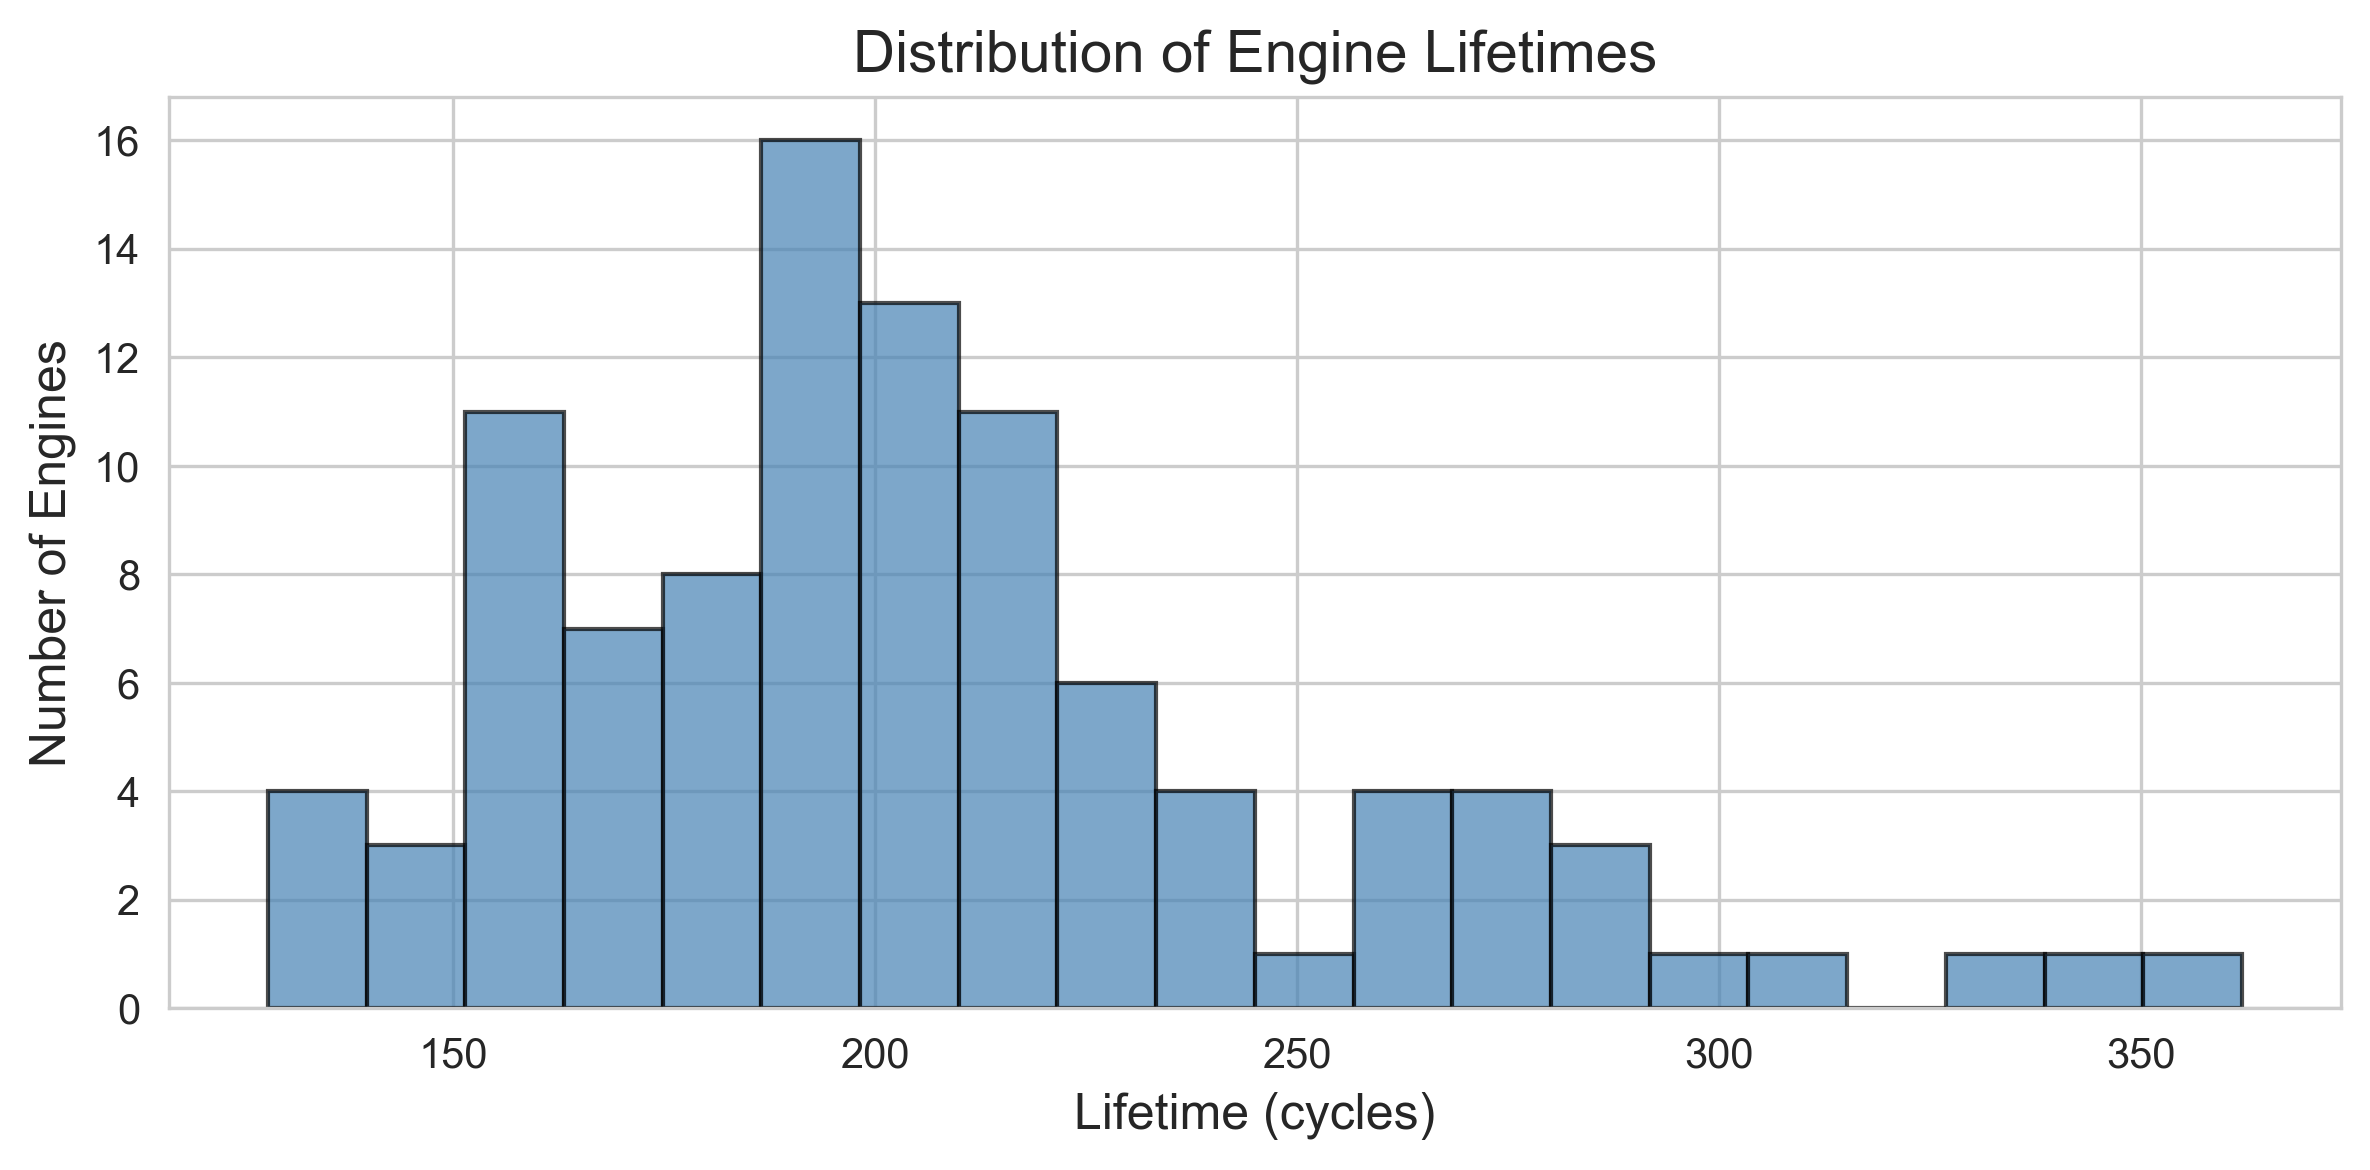
\includegraphics[width=0.75\textwidth]{fig_lifetime_dist.png}
\caption{Distribution of engine lifetimes in the FD001 training set.}
\label{fig:lifetime}
\end{figure}

Not all 21 sensors are equally informative. Figure~\ref{fig:sensor_corr} shows the Pearson correlation of each sensor with RUL. Several sensors (e.g., sensors 2, 3, 4, 11, 15) show strong negative correlations, indicating clear degradation trends. Others (e.g., sensors 1, 5, 10, 16) show near-zero correlation and are effectively constant.

\begin{figure}[H]
\centering
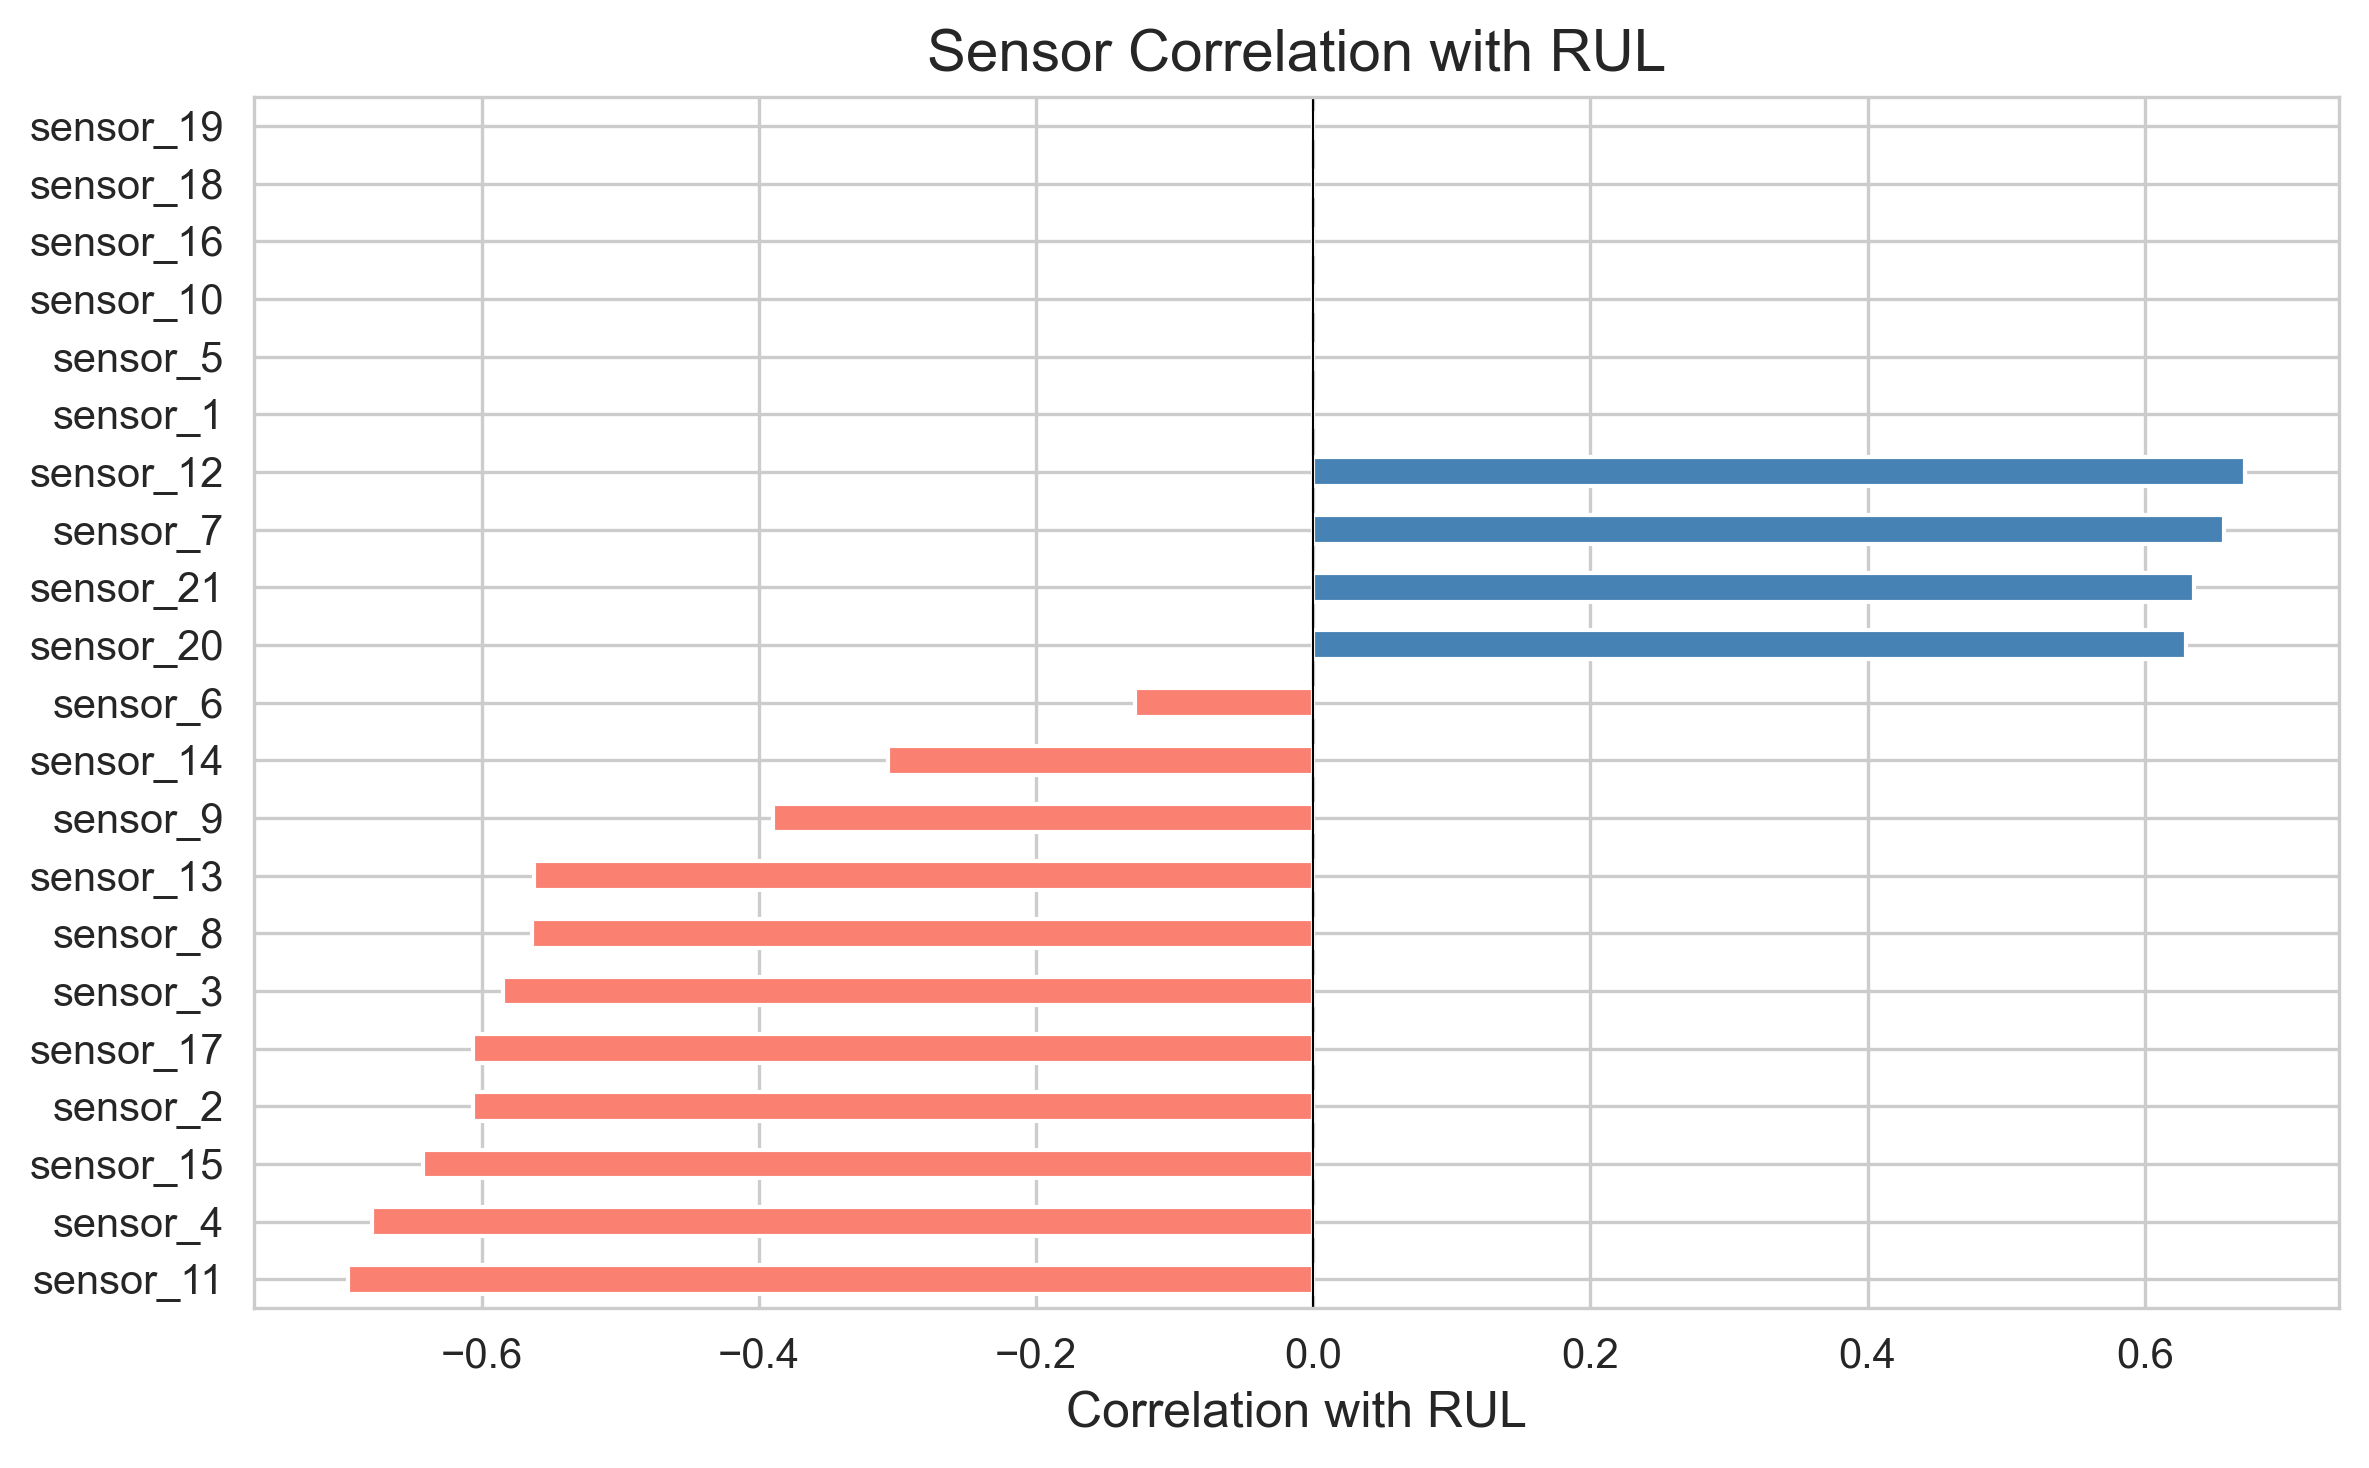
\includegraphics[width=0.75\textwidth]{fig_sensor_corr.png}
\caption{Correlation of each sensor measurement with RUL.}
\label{fig:sensor_corr}
\end{figure}

% ============================================================
\section{Methodology}

\subsection{Feature Engineering}

We apply three preprocessing steps:

\begin{enumerate}[nosep]
    \item \textbf{Constant column removal}: 8 features with near-zero variance (setting\_2, setting\_3, sensors 1, 5, 10, 16, 18, 19) are removed, leaving 16 informative features.
    \item \textbf{RUL clipping at 125 cycles}: Early in an engine's life, degradation is not yet detectable by sensors. Following standard practice, we cap the RUL target at 125, creating a piecewise-linear label (constant at 125 for healthy operation, then linearly decreasing). This focuses model learning on the degradation region. Figure~\ref{fig:rul_clip} illustrates this transformation.
    \item \textbf{MinMax normalization}: All features are scaled to $[0, 1]$ to ensure no single sensor dominates due to scale differences.
\end{enumerate}

\begin{figure}[H]
\centering
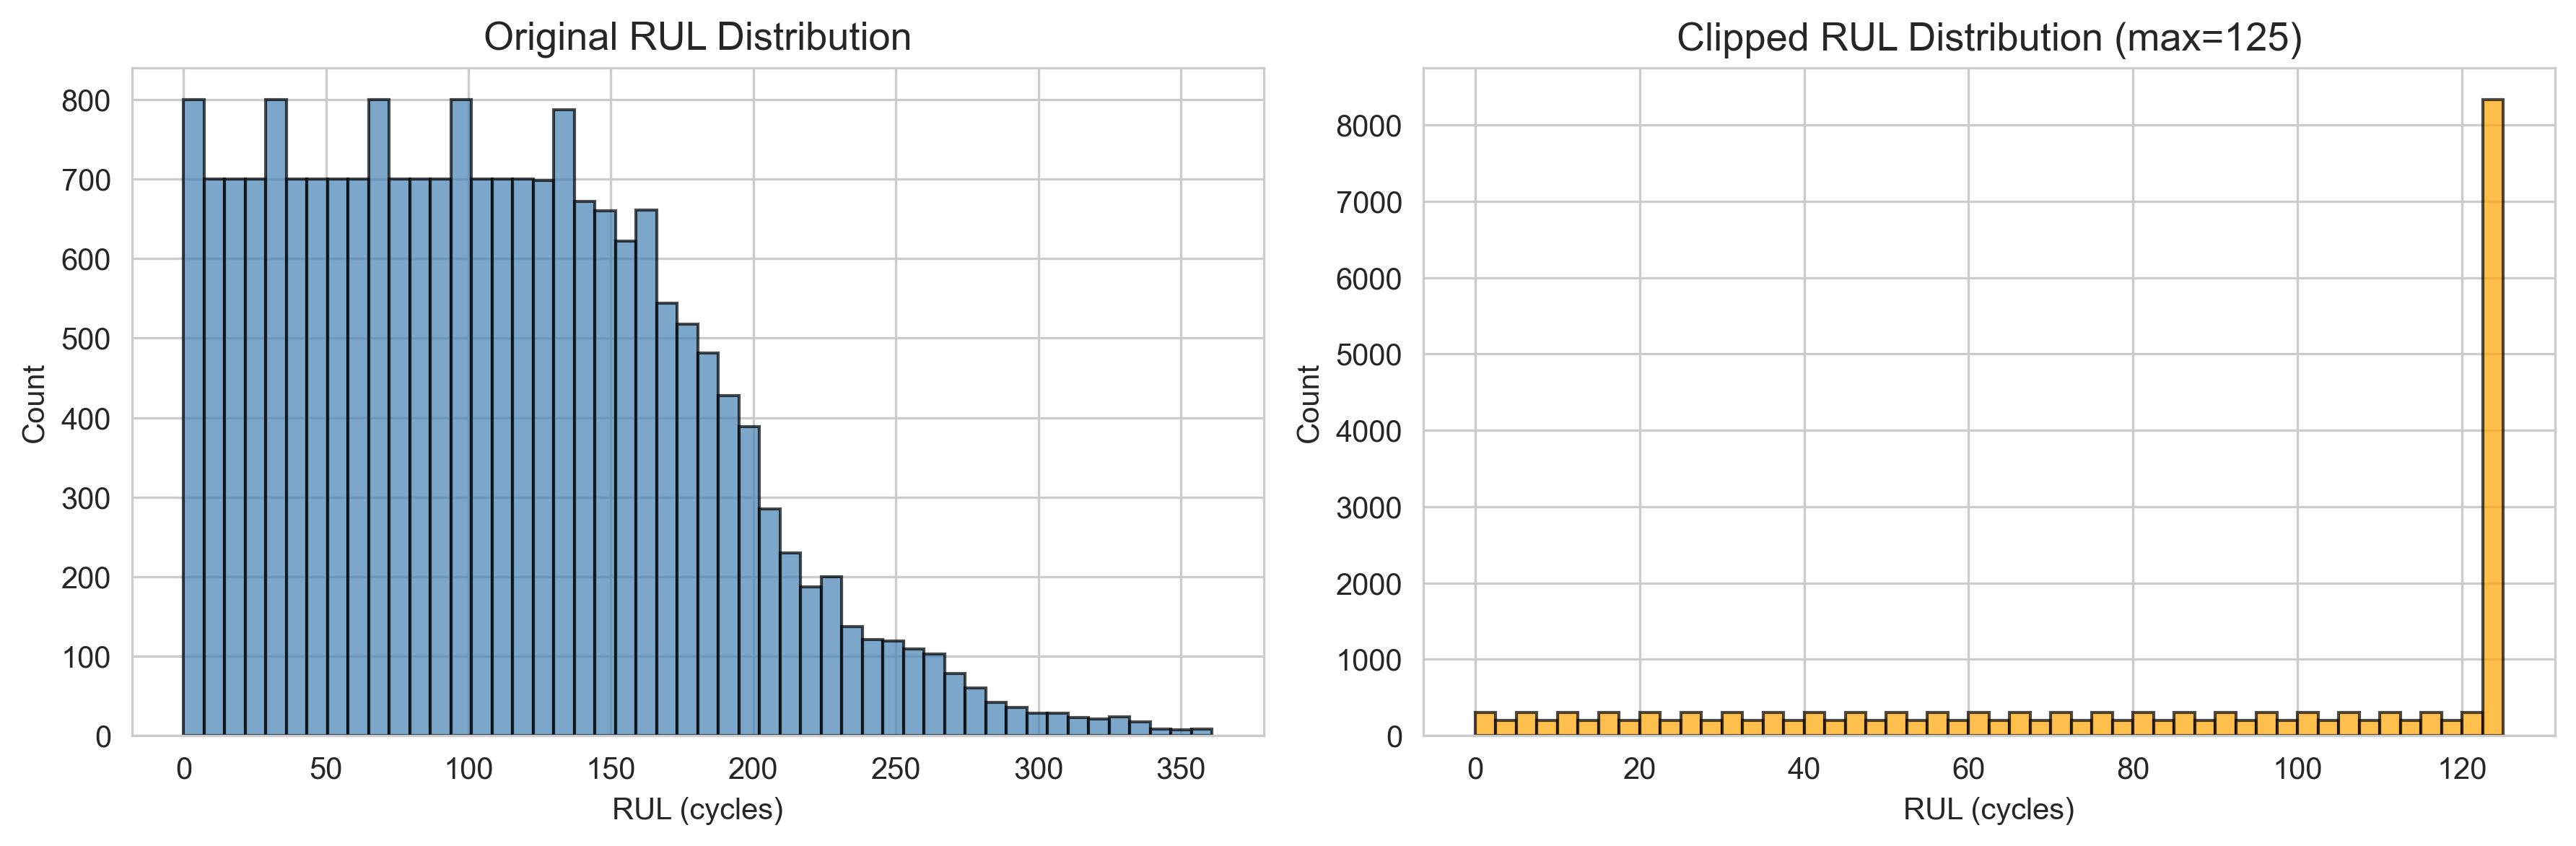
\includegraphics[width=0.85\textwidth]{fig_rul_clip.png}
\caption{Original vs.\ clipped RUL distribution. Clipping at 125 cycles concentrates labels in the degradation region.}
\label{fig:rul_clip}
\end{figure}

\subsection{Sensor Degradation Patterns}

Figure~\ref{fig:trends} shows the average degradation trends for the six most correlated sensors. Each plot shows the mean sensor value ($\pm$1 standard deviation) across all engines as a function of RUL. Clear monotonic trends near failure (right side) confirm that these sensors carry strong prognostic signals.

\begin{figure}[H]
\centering
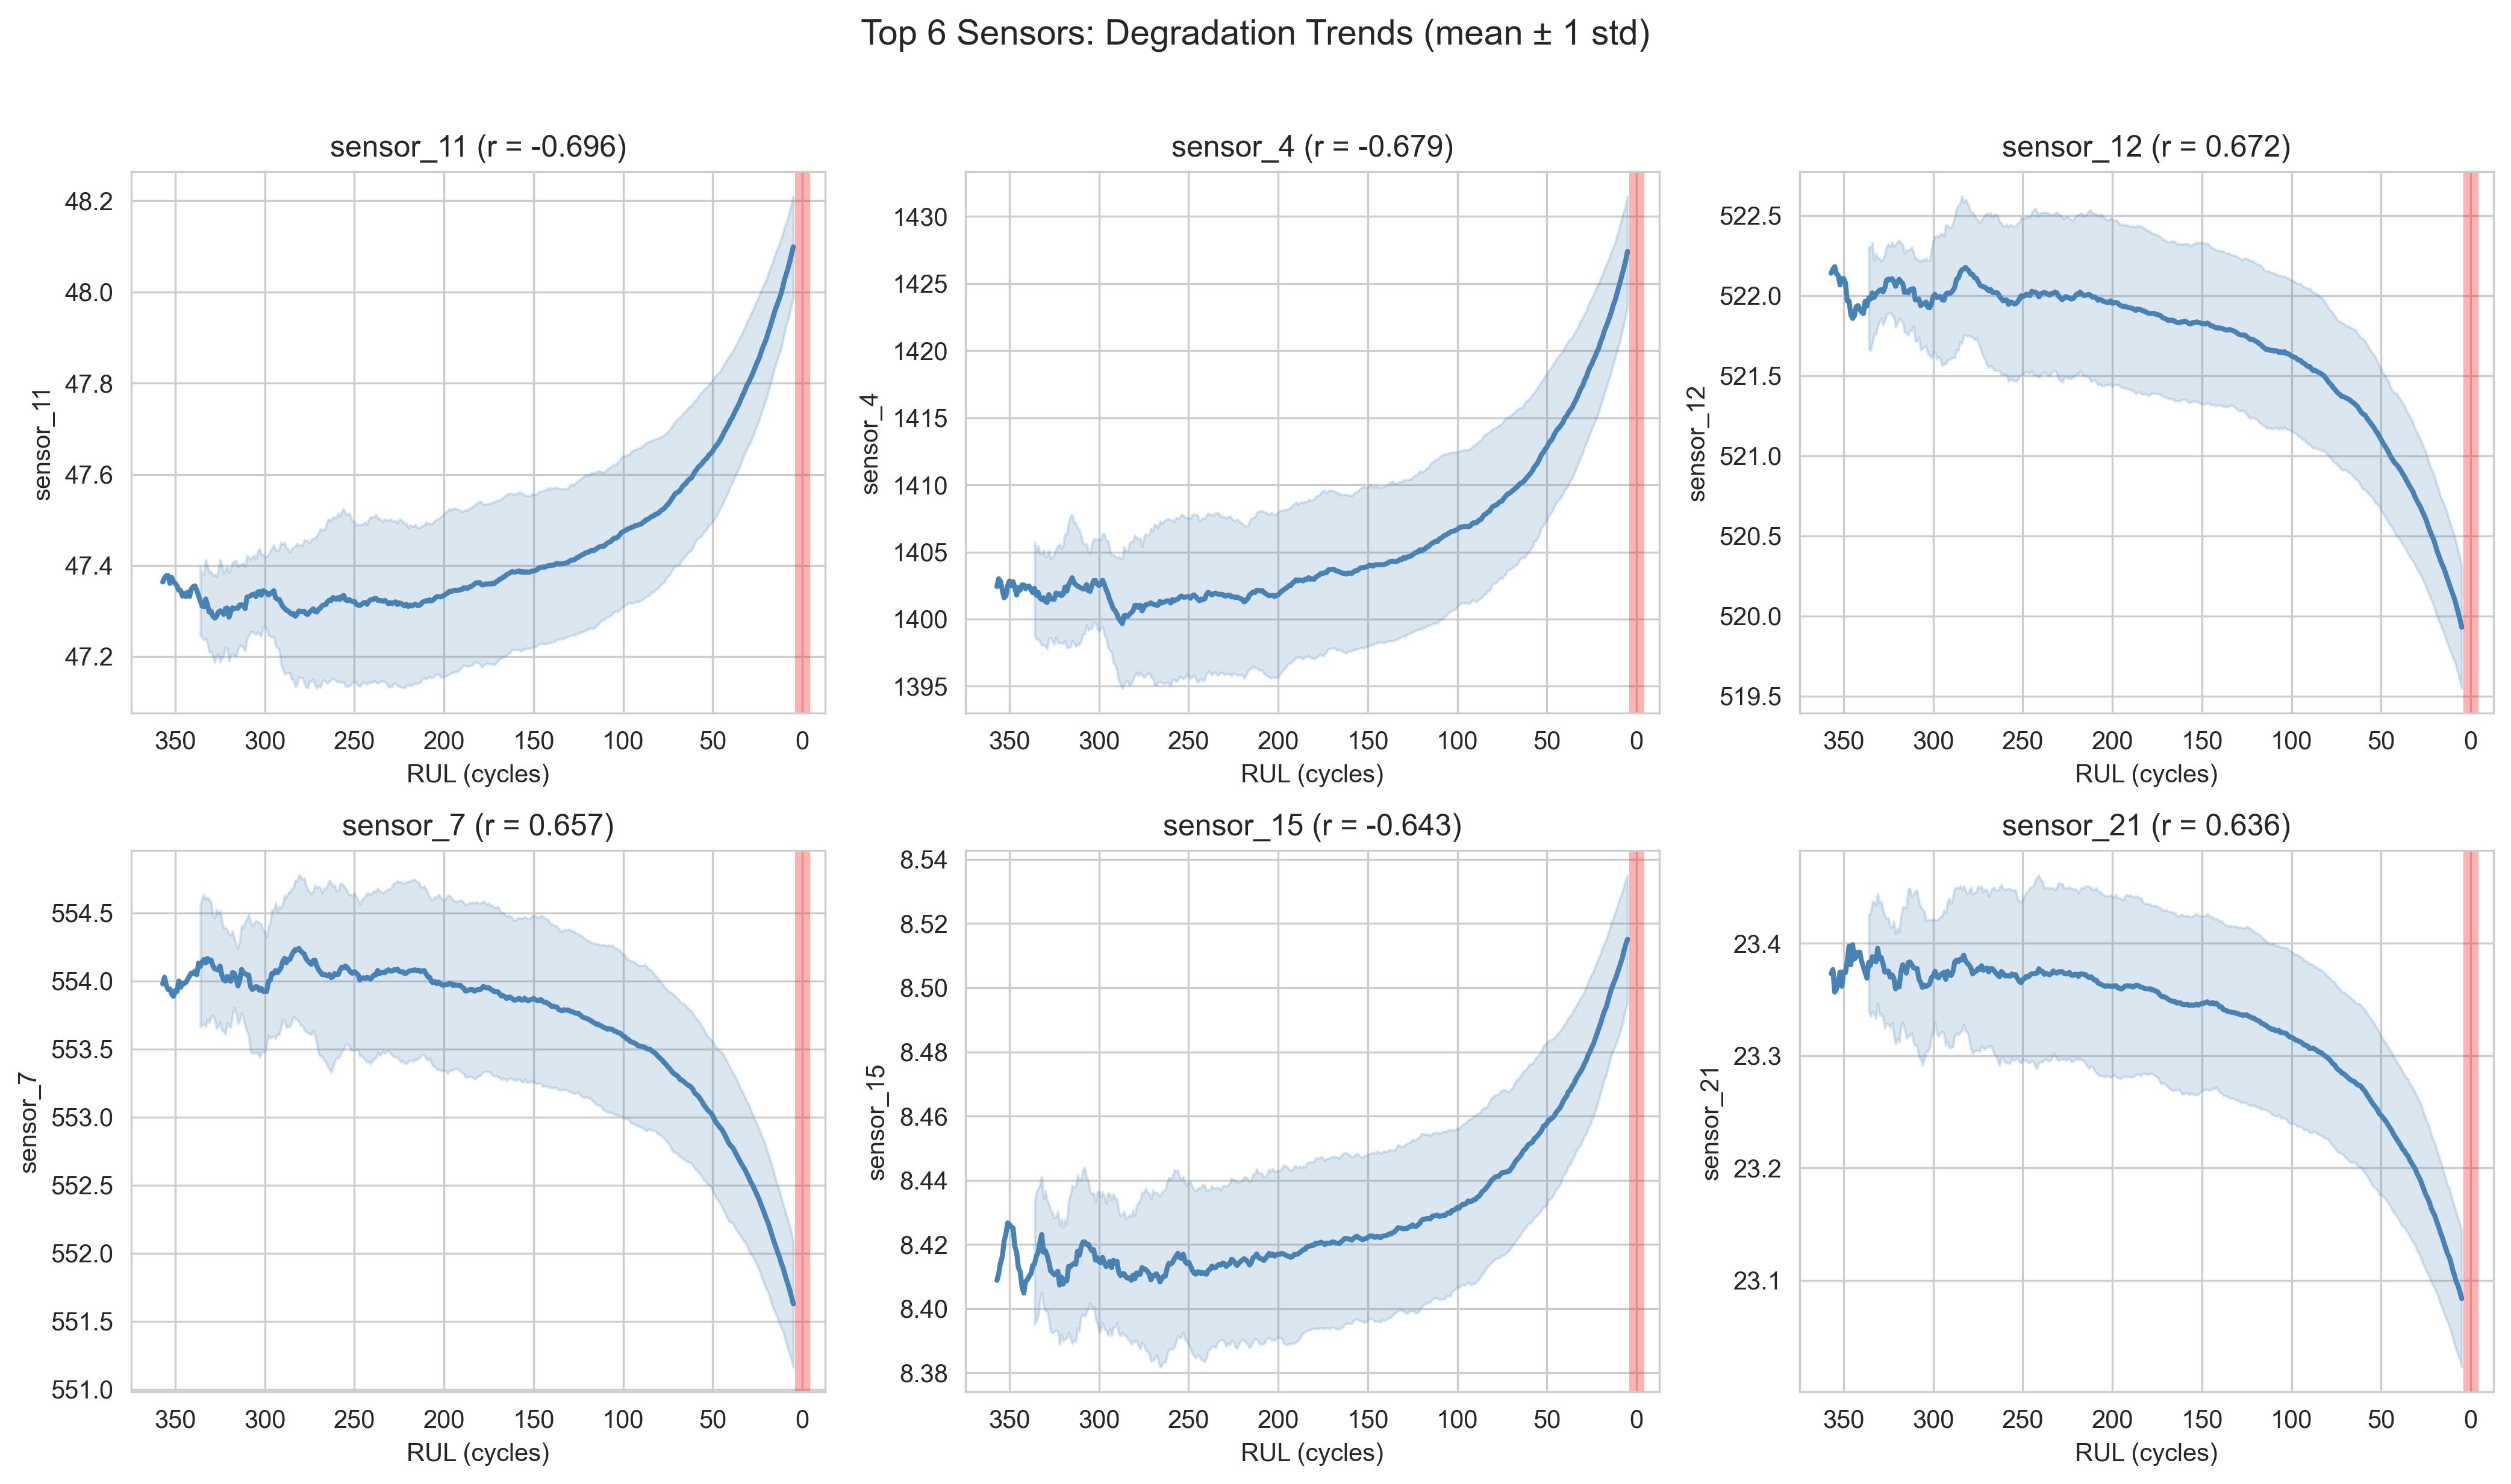
\includegraphics[width=0.95\textwidth]{fig_sensor_trends.png}
\caption{Degradation trends for the top 6 sensors by absolute correlation with RUL. X-axis shows cycles remaining until failure.}
\label{fig:trends}
\end{figure}

\subsection{Models}

We evaluate three regression models:

\begin{itemize}[nosep]
    \item \textbf{Linear Regression (LR)}: A baseline that assumes a linear relationship between features and RUL.
    \item \textbf{Random Forest (RF)}: An ensemble of 100 decision trees that captures nonlinear relationships through bagging.
    \item \textbf{XGBoost}: A gradient-boosted tree ensemble (100 trees, learning rate 0.1) that iteratively corrects prediction errors.
\end{itemize}

All models are trained on an 80/20 random split of the training data (16{,}504 training / 4{,}127 validation samples) with a fixed random seed for reproducibility.

% ============================================================
\section{Results}

\subsection{Validation Set Comparison}

Table~\ref{tab:val_results} compares the three models on the validation set. Both tree-based models substantially outperform Linear Regression, and XGBoost achieves the lowest RMSE and MAE.

\begin{table}[H]
\centering
\caption{Validation Set Performance}
\label{tab:val_results}
\begin{tabular}{lccc}
\toprule
\textbf{Model} & \textbf{RMSE} & \textbf{MAE} & $\boldsymbol{R^2}$ \\
\midrule
Linear Regression & 21.68 & 17.61 & 0.723 \\
Random Forest     & 18.77 & 13.58 & 0.792 \\
XGBoost           & 18.72 & 13.31 & 0.793 \\
\bottomrule
\end{tabular}
\end{table}

\subsection{Test Set Results}

Using XGBoost as the best model, we evaluate on the held-out test set (100 engines, predicting RUL at the last observed cycle). Table~\ref{tab:test_results} shows the results.

\begin{table}[H]
\centering
\caption{Test Set Performance (XGBoost)}
\label{tab:test_results}
\begin{tabular}{lccc}
\toprule
\textbf{Model} & \textbf{RMSE} & \textbf{MAE} & $\boldsymbol{R^2}$ \\
\midrule
XGBoost & 16.73 & 11.83 & 0.826 \\
\bottomrule
\end{tabular}
\end{table}

The test RMSE of 16.73 cycles is notably lower than the validation RMSE (18.72), likely because the test set evaluates only the last cycle per engine (a single prediction per trajectory) rather than all time steps including early, high-RUL samples.

\subsection{Feature Importance}

Figure~\ref{fig:importance} shows the XGBoost feature importance. Sensors 11, 4, and 9 are the most important predictors, consistent with their strong correlation with RUL observed in the exploratory analysis.

\begin{figure}[H]
\centering
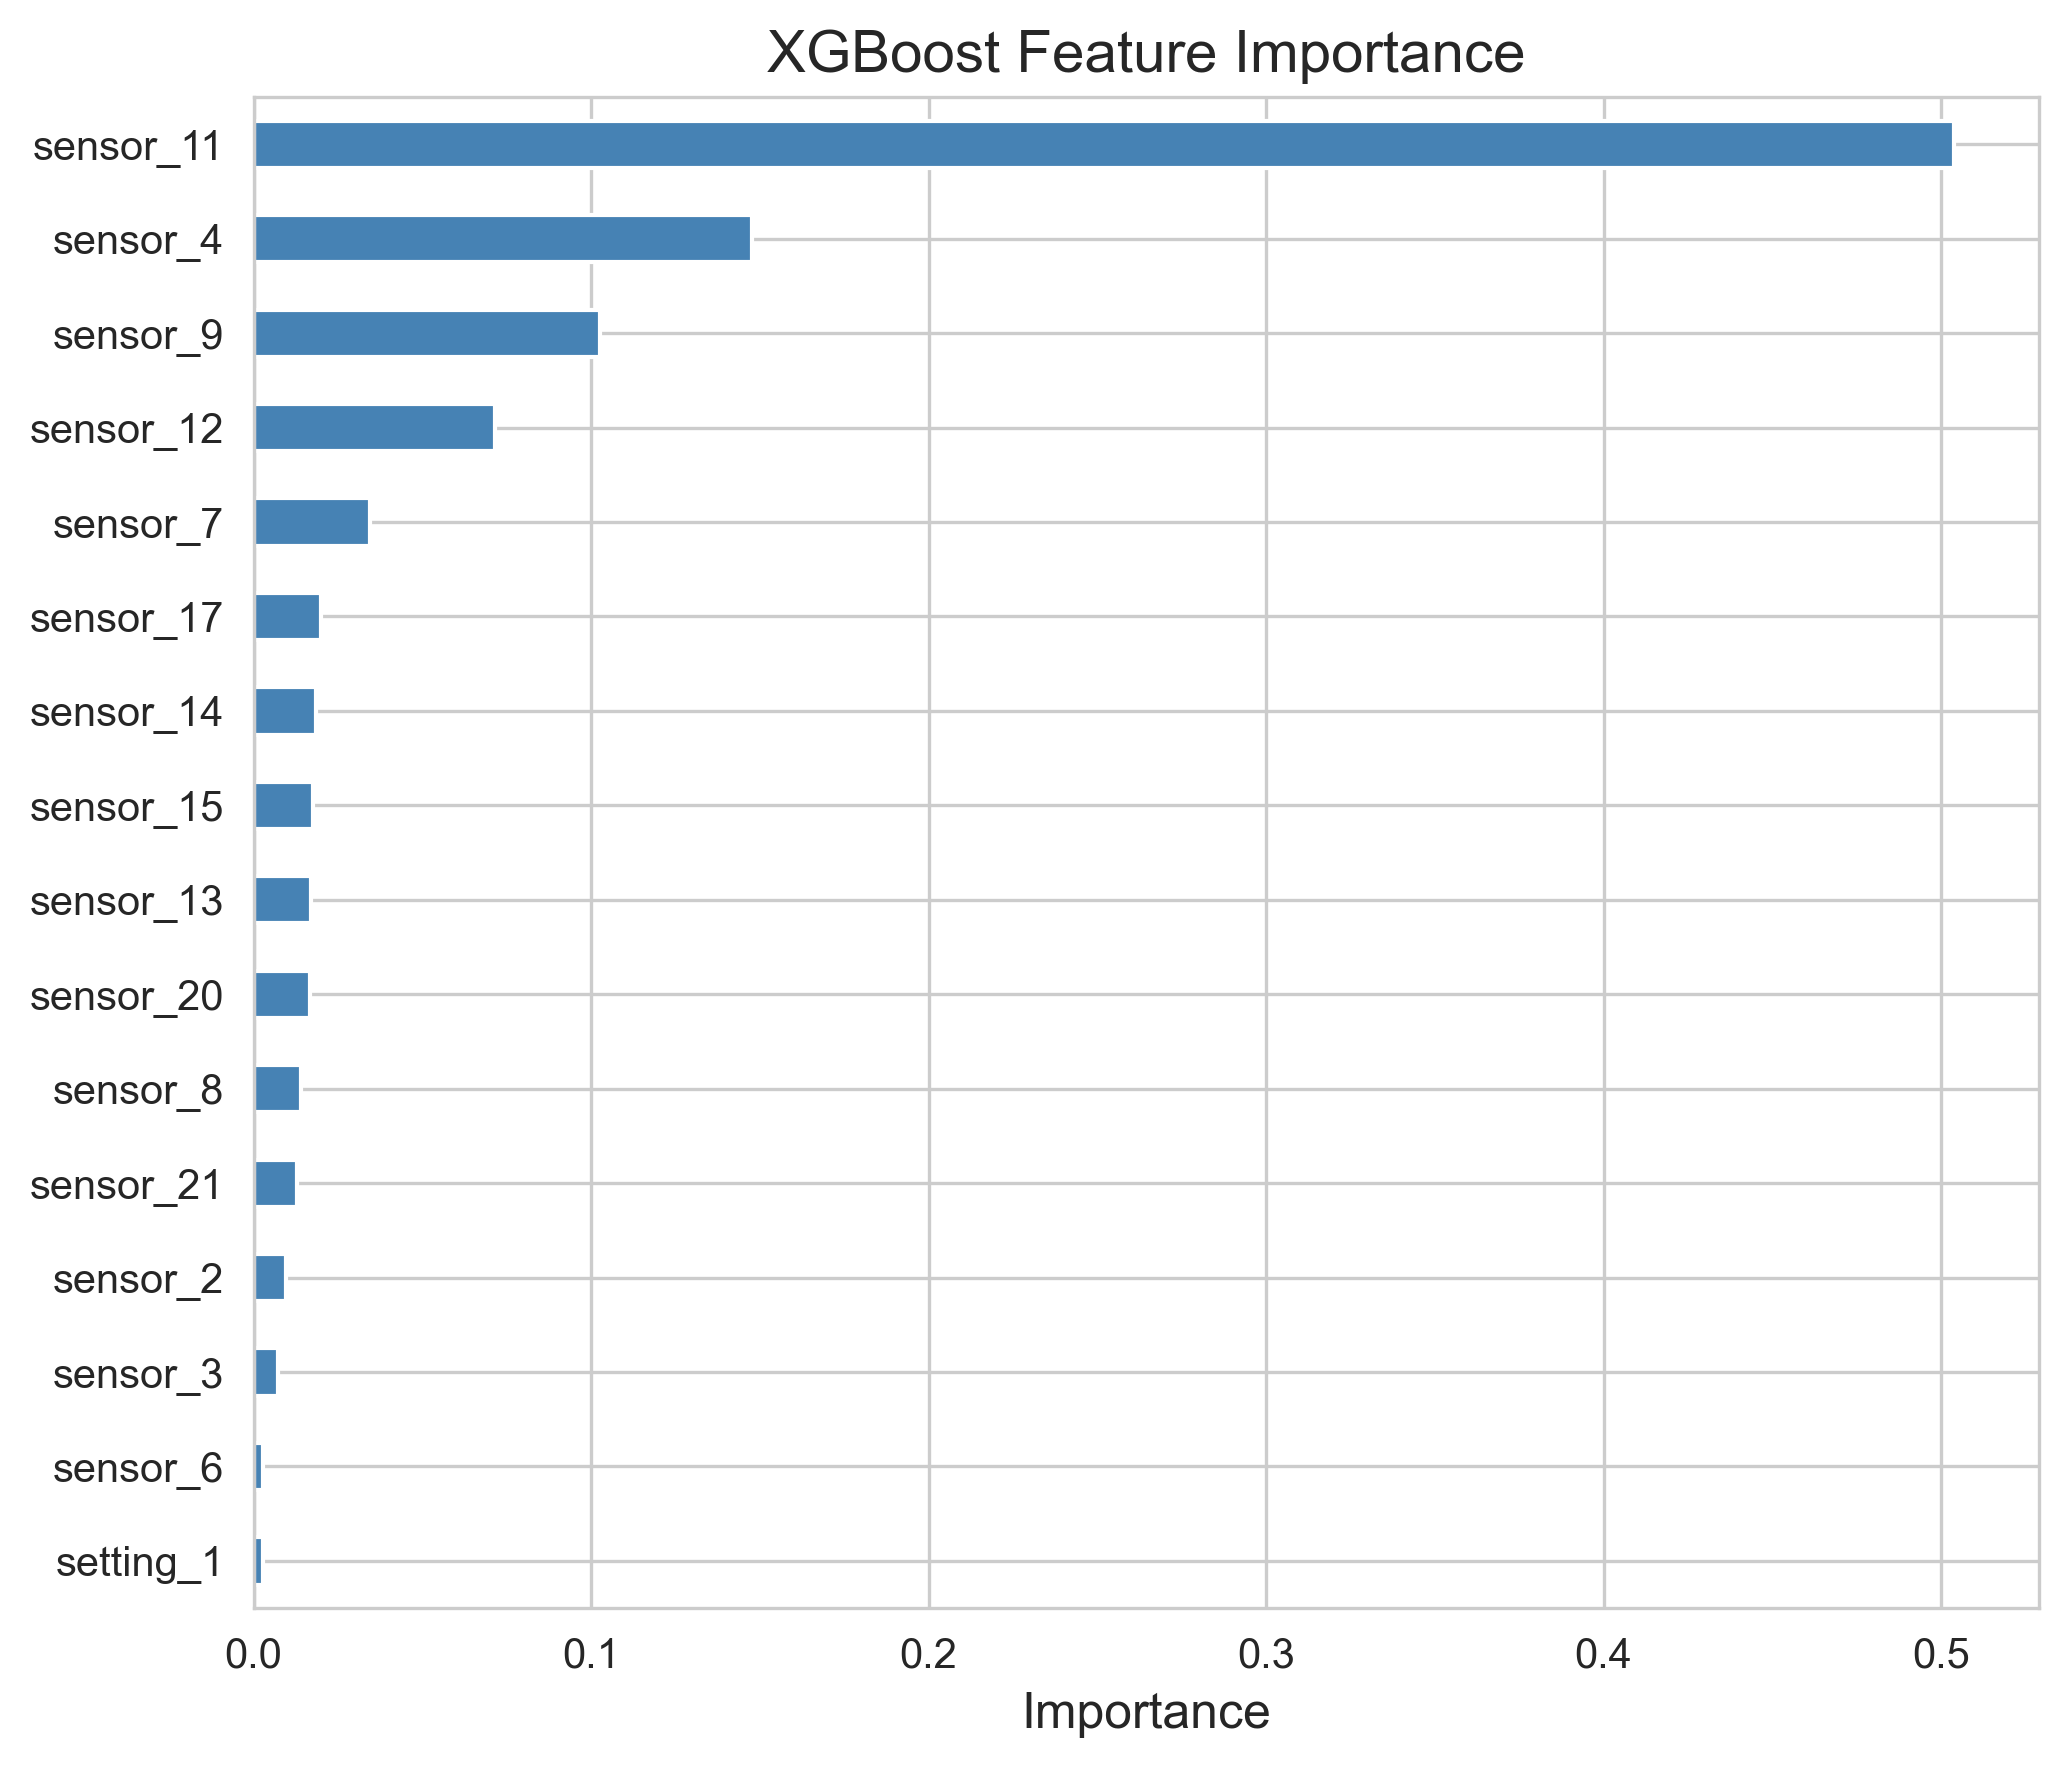
\includegraphics[width=0.65\textwidth]{fig_feature_importance.png}
\caption{XGBoost feature importance ranking.}
\label{fig:importance}
\end{figure}

\subsection{Predicted vs.\ Actual RUL}

Figure~\ref{fig:scatter} shows the predicted vs.\ actual RUL for the 100 test engines. Points cluster near the diagonal, indicating good prediction accuracy. The model performs well across the full RUL range, with slightly more scatter at high RUL values where degradation signals are weaker.

\begin{figure}[H]
\centering
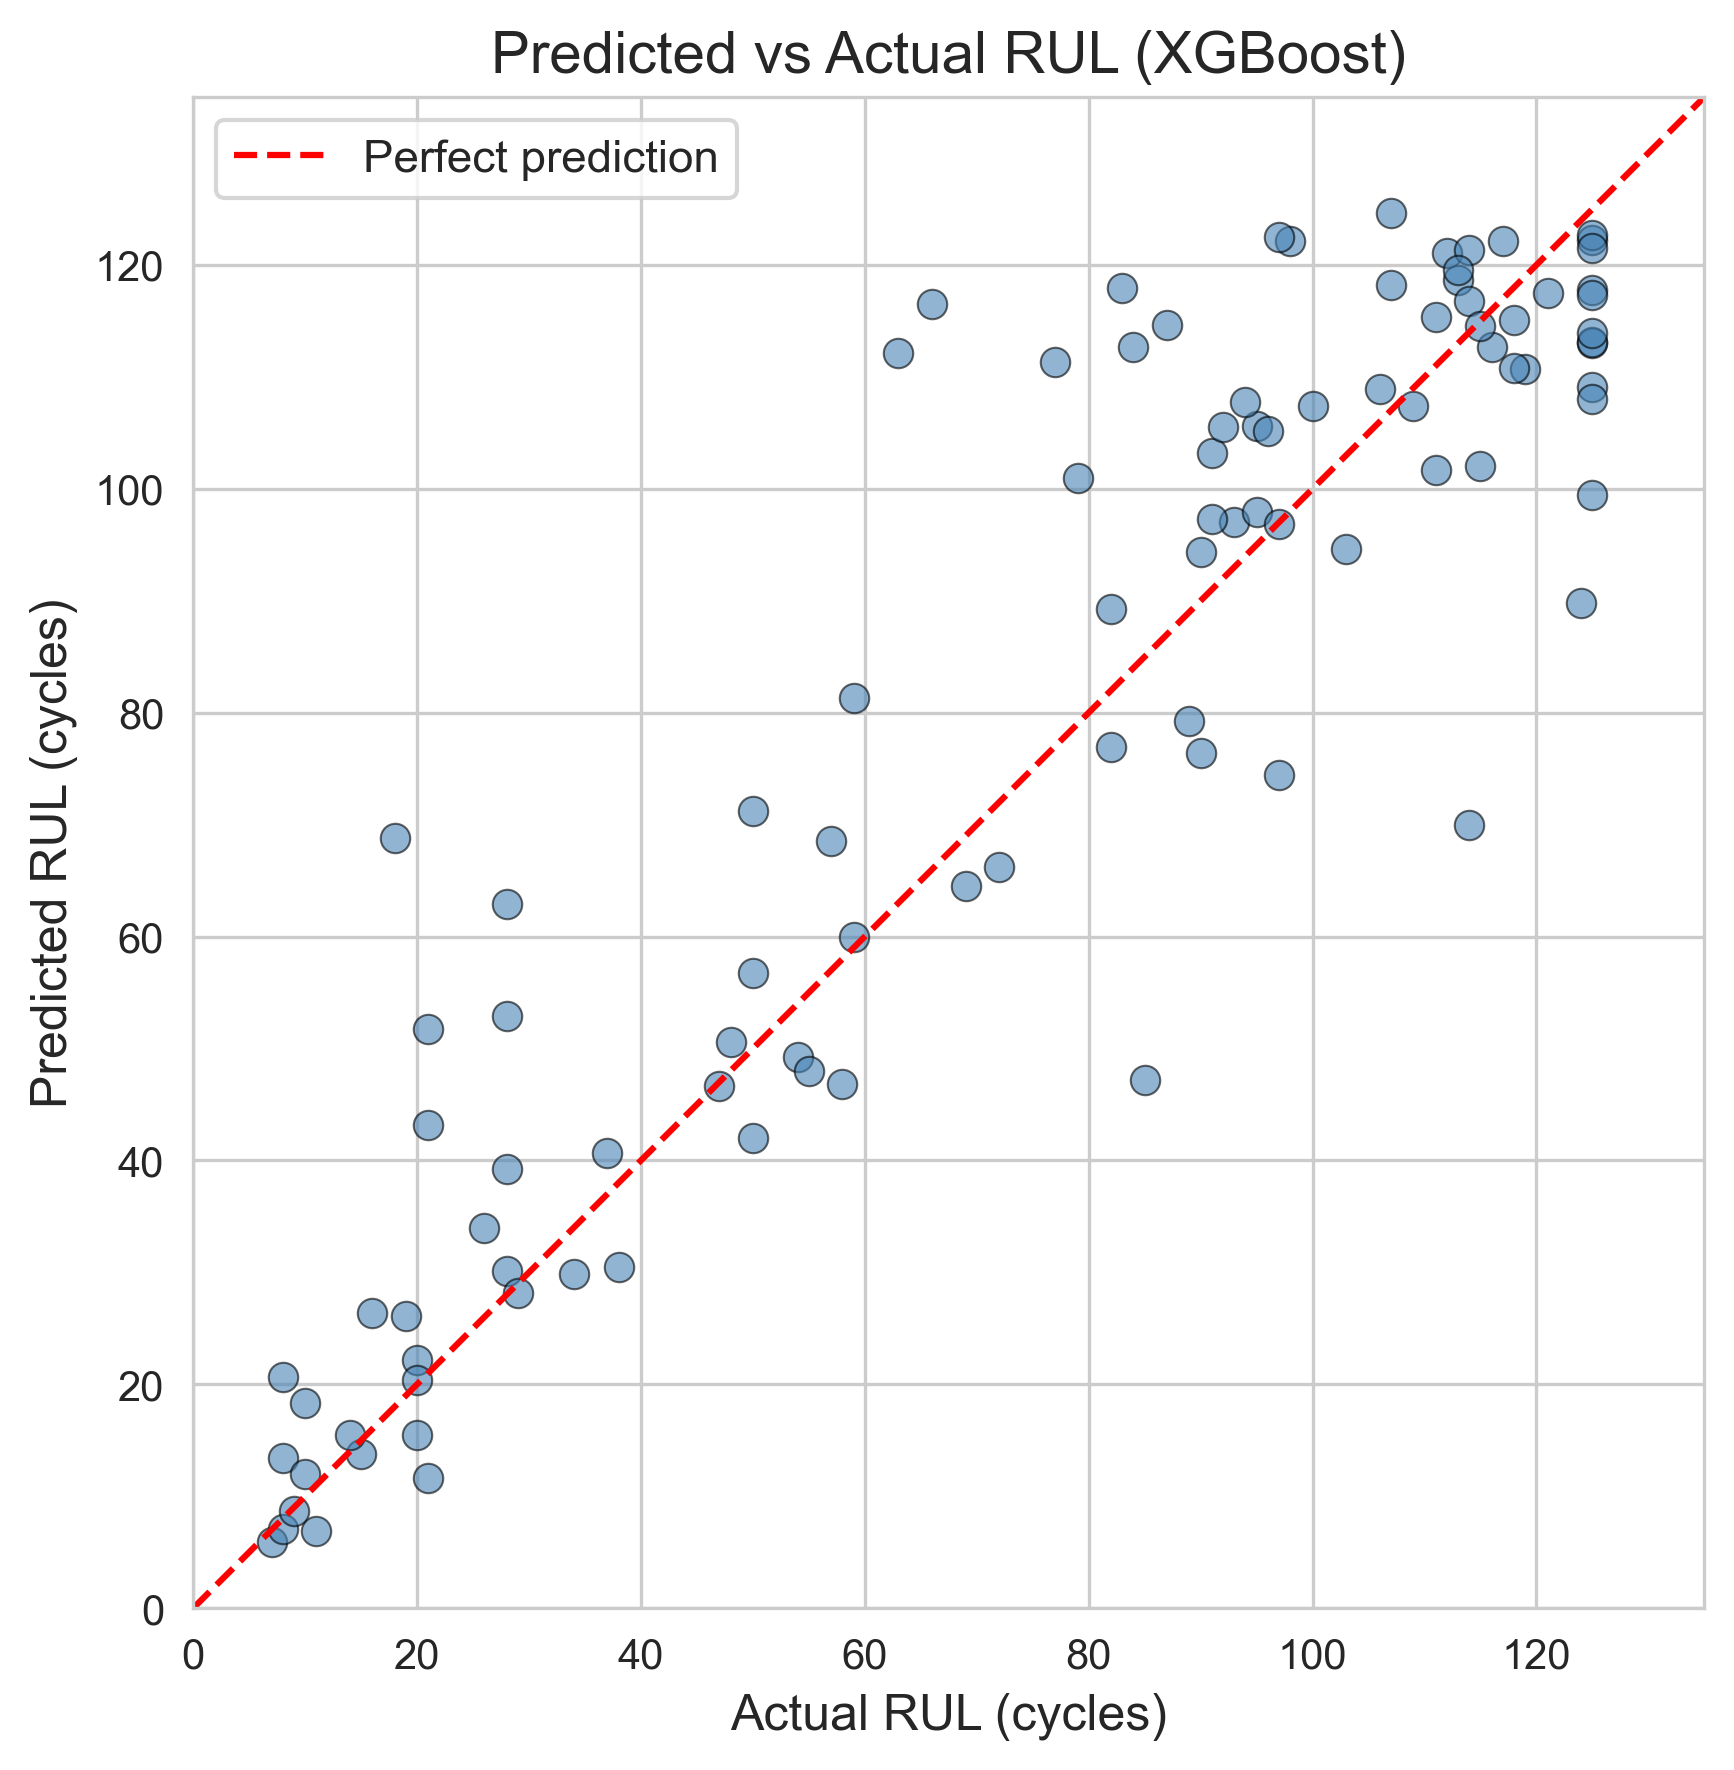
\includegraphics[width=0.55\textwidth]{fig_pred_vs_actual.png}
\caption{Predicted vs.\ actual RUL on the test set. The dashed red line indicates perfect prediction.}
\label{fig:scatter}
\end{figure}

% ============================================================
\section{Conclusion}

This study demonstrates that machine learning models can effectively predict turbofan engine RUL from multivariate sensor data. Key findings:

\begin{itemize}[nosep]
    \item XGBoost achieves the best performance (test RMSE = 16.73, $R^2$ = 0.826), outperforming both Linear Regression and Random Forest.
    \item Simple preprocessing---removing constant sensors, clipping RUL at 125, and MinMax normalization---is sufficient for strong baseline performance.
    \item Sensors 11, 4, and 9 are the most important features, showing clear degradation trends as engines approach failure.
\end{itemize}

\textbf{Limitations.} The FD001 dataset represents a single operating condition and fault mode. Real-world engines operate under varying conditions (addressed by FD002--FD004 datasets). The current approach treats each time step independently, ignoring temporal dependencies within engine trajectories.

\textbf{Future work.} Recurrent neural networks (e.g., LSTM) or temporal convolutional networks could capture sequential degradation patterns. Extending the analysis to multi-condition datasets (FD002--FD004) would test model robustness. Additionally, incorporating a scoring function that penalizes late predictions more heavily than early ones would better reflect real-world maintenance priorities.

\end{document}
